\documentclass{article}
\usepackage{xeCJK}
\usepackage{amsmath}
\usepackage{amssymb}
\usepackage{mathrsfs}
\usepackage{bm}
\usepackage{hyperref}
\usepackage{graphicx}
\usepackage{float}
\usepackage[ruled,linesnumbered]{algorithm2e}

\setlength{\parindent}{2em}
\usepackage{geometry}
\geometry{a4paper, left=2.54cm, right=2.54cm, top=3.18cm, bottom=3.18cm}

% 设置文章行距
\renewcommand{\baselinestretch}{1.5}

% 定义引用格式
% \newcommand{\myeqref}[1]{\eqref{#1}式}
% \newcommand{\figref}[1]{图\ref{#1}}
% \newcommand{\tabref}[1]{表\ref{#1}}

\begin{document}


\section{局部耦合中跨边界坐标的调整}

\begin{figure}[htbp]
    \centering
    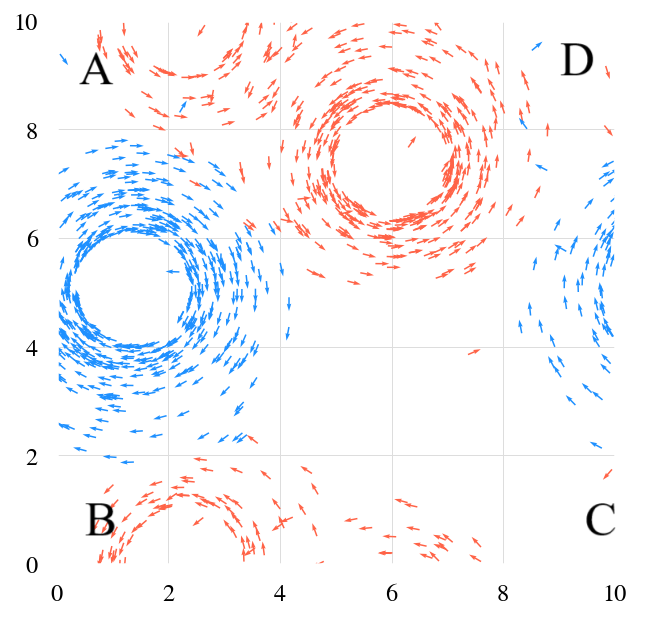
\includegraphics[width=0.4\textwidth]{./figs/fig1.jpg}
    \caption{跨边界坐标的调整}
    \label{fig:fig22}
\end{figure}

给定$(x_i, y_i)$, 对于任意的$(x_j, y_j)$, 做如下变换

\begin{equation}\label{eq:eq1}
	\bar{x}_j=\begin{cases}
		x_j,&		|x_i-x_j|\le L/2\\
		x_j+L,&		x_i-x_j>L/2\\
		x_j-L,&		x_j-x_i>L/2\\
	\end{cases} ,\quad
	\bar{y}_j=\begin{cases}
		y_j,&		|y_i-y_j|\le L/2\\
		y_j+L,&		y_i-y_j>L/2\\
		y_j-L,&		y_j-y_i>L/2\\
	\end{cases}
\end{equation}

其中,$L$为边界长度. 例如,对于\ref{fig:fig22}中的情况,以A为$(x_i, y_i)$时,B需调整纵坐标,D需调整横坐标,C需同时调整横纵坐标.

$\ $

原始距离为

$$
d_{ij}=\sqrt{(x_i-x_j)^2+(y_i-y_j)^2}
$$

变换后的距离为

$$
\bar{d}_{ij}=\sqrt{(x_i-\bar{x}_j)^2+(y_i-\bar{y}_j)^2}
$$

下证$\bar{d}_{ij} \le d_{ij}$, 即调整后的距离不会大于原始距离.

$ $

对于$(x_i-x_j)^2, (x_i-\bar{x}_j)^2$, 若$x_i\ne \bar{x}_j$,有

$$
\begin{array}{l}
	(x_i-\bar{x}_j)^2-(x_i-x_j)^2\\
	=\left( x_j\pm L-x_i \right) ^2-(x_i-x_j)^2\\
	=L^2\pm 2L\left( x_j-x_i \right)\\
	=\left\{ \begin{matrix}
	L^2+2L\left( x_j-x_i \right) ,&		x_i-x_j>5\\
	L^2-2L\left( x_j-x_i \right) ,&		x_j-x_i>5\\
\end{matrix} \right.\\
	<L^2-10L\\
	=0, \left( L=10 \right)\\
\end{array}
$$

即

$$
(x_i-\bar{x}_j)^2<(x_i-x_j)^2, \left( L=10, x_i\ne \bar{x}_j \right)
$$

同理可证

$$
(y_i-\bar{y}_j)^2<(y_i-y_j)^2, \left( L=10, x_i\ne \bar{x}_j \right)
$$

综上有

$$
\bar{d}_{ij}=\sqrt{(x_i-\bar{x}_j)^2+(y_i-\bar{y}_j)^2}\le \sqrt{(x_i-x_j)^2+(y_i-y_j)^2}=d_{ij}
$$

当且仅当$x_i=\bar{x}_j$且$y_i=\bar{y}_j$时,取等号.

因此

$$
\begin{aligned}
	D_{ij}&=\min \left\{ \sqrt{(x_i-\bar{x}_j)^2+(y_i-\bar{y}_j)^2},\sqrt{(x_i-x_j)^2+(y_i-y_j)^2} \right\}\\
	&=\sqrt{(x_i-\bar{x}_j)^2+(y_i-\bar{y}_j)^2}\\
\end{aligned}
$$

\newpage

\section{相位-取向关联的集群振子系统的动力学研究}

\textbf{$\Delta$ 聚焦点}
\begin{enumerate}
    \item 环态及其相变
    \item 环态的解域与相位同步的关系
    \item 数值结果的细致讨论, 分类
    \item 必要的理论分析与估计
\end{enumerate}

分析点
\subsection{单个粒子的运动问题(无相互作用)}

$$
\begin{cases}
	\begin{array}{c}
	\Delta x\left( t \right) =v\cos \theta \Delta t\\
	\Delta y\left( t \right) =v\sin \theta \Delta t\\
\end{array}\rightarrow \begin{array}{c}
	\dot{x}=v\cos \theta\\
	\dot{y}=v\sin \theta\\
\end{array}\\
	\dot{\theta}_i=\omega _i\rightarrow \theta _i\left( t \right) =\omega _it\\
	v=\sqrt{\dot{x}_{i}^{2}+\dot{y}_{i}^{2}}=v\left( constant \right)\\
\end{cases}
$$

运动半径 $=\ ?$

$$
\begin{cases}
	x_i\left( t \right) =x_i\left( 0 \right) -\frac{v}{\omega _i}\sin \omega _it\\
	y_i\left( t \right) =y_i\left( 0 \right) -\frac{v}{\omega _i}\cos \omega _it\\
\end{cases}
$$

$$
\Rightarrow \left( x_i-x_{i}^{0} \right) ^2+\left( y_i-y_{i}^{0} \right) ^2=\left( \frac{v}{\omega _i} \right) ^2
$$

每个粒子的运动轨迹是一个圆,圆心为 $\left( x_i^0,y_i^0 \right)$,半径为 $\frac{v}{\omega _i}$

\subsection{考虑相互作用$\lambda$,耦合距离$d_0$ ($\{A_ij\}$,注意是时变的)}

\begin{itemize}
    \item 看空间聚集过程
    \item 空间尺度也考虑进去
\end{itemize}

粒子数$N$,$L\times L\sim \sqrt{\frac{L\times L}{N}}\sim \frac{L}{\sqrt{N}}$

\begin{enumerate}
    \item 每个单粒子的运动空间尺度, $\cfrac{v}{\omega_i}$
    \item 耦合距离 $d_0$
    \item 粒子平均间距 $\cfrac{L}{\sqrt{N}}$
\end{enumerate}

$$
d_0\sim \frac{L}{\sqrt{N}}\rightarrow d_0\ll \frac{L}{\sqrt{N}}, d_0\gg \frac{L}{\sqrt{N}}
$$

低频粒子:$d_0\ll \frac{v}{\omega _i}$
高频粒子:$d_0\gg \frac{v}{\omega _i}$

在计算空间pattern同时,还要跟踪每个粒子的相速度$\dot{\theta}_i(t)$

\subsection{序参量 Order Parameter}

\subsubsection{相位单位圆}

由于粒子数较多,为了更清晰地刻画粒子相位的同步情况,绘制三维空间中的单位圆. 将单位圆等分为$M$个区间,每个区间的大小为$\frac{2\pi}{M}$,$z$轴表示单位圆上相位处于该区间的粒子数,类似于分布.

\begin{figure}[H]
	\centering
	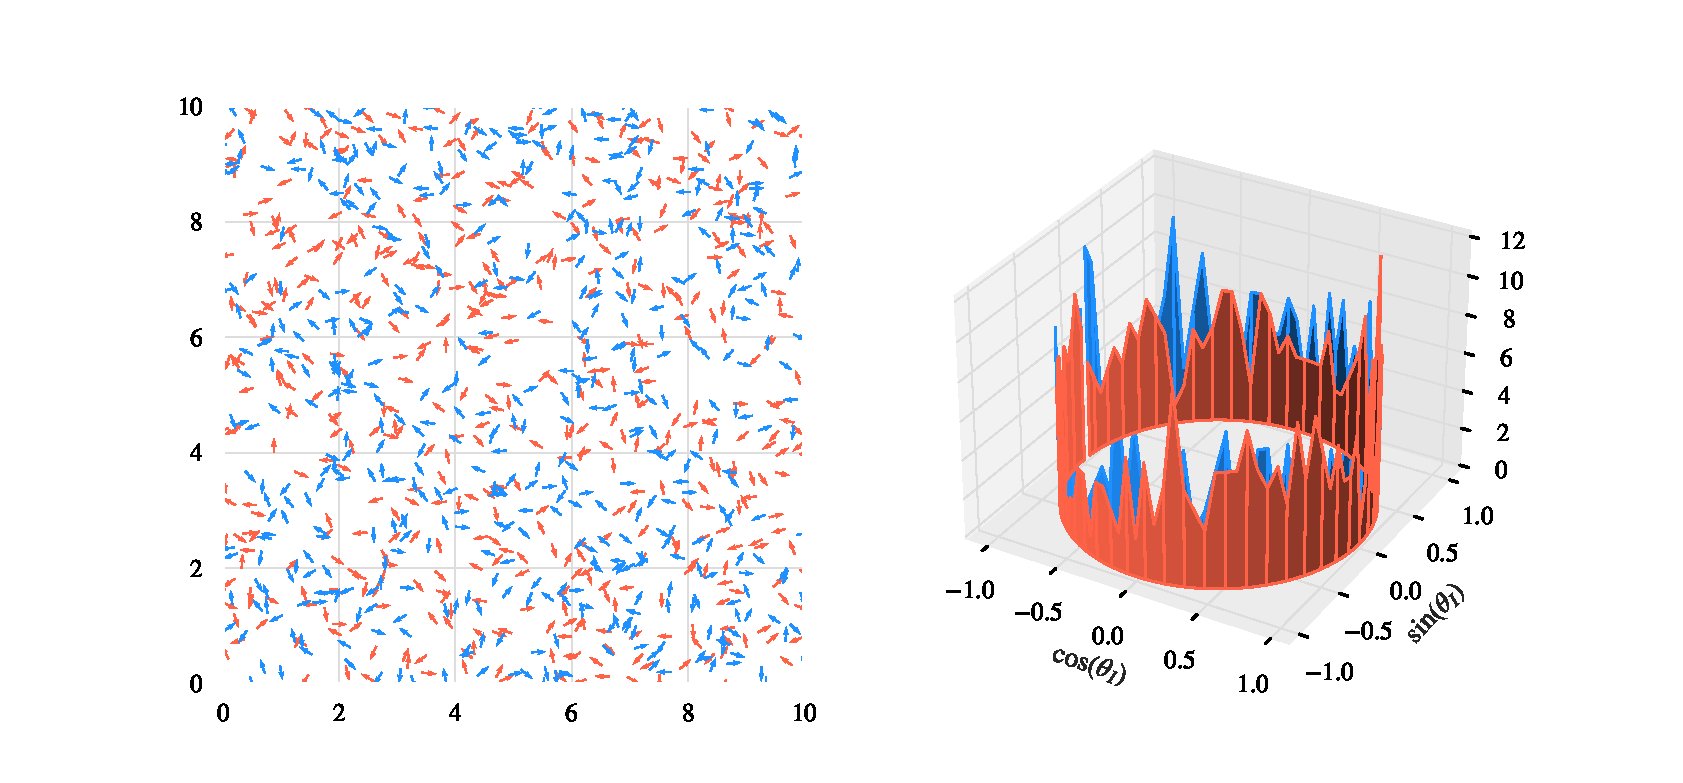
\includegraphics[width=\textwidth]{./figs/CorrectCoupling_uniform_0.010_0.10.eps}
	\vspace{-1cm}
	\caption{混沌态 ($\lambda=0.01, d_0=0.1, random seed=10$)}
	\label{fig:fig231.1}
\end{figure}

\begin{figure}[H]
	\centering
	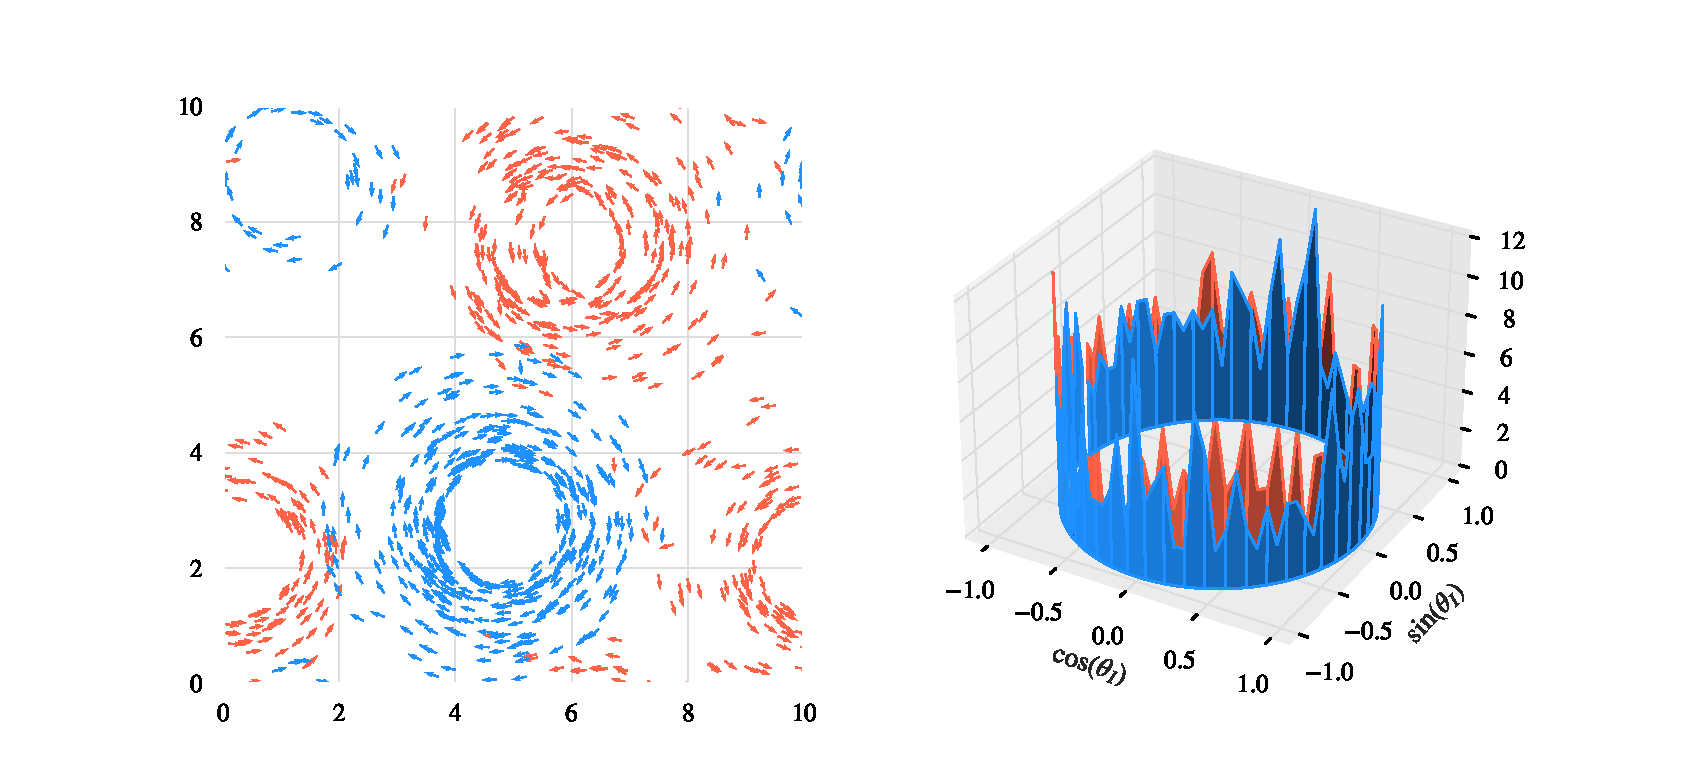
\includegraphics[width=\textwidth]{./figs/CorrectCoupling_uniform_0.020_0.30.eps}
	\vspace{-1cm}
	\caption{环态 ($\lambda=0.02, d_0=0.3, random seed=10$)}
	\label{fig:fig231.2}
\end{figure}

当粒子处于混沌态或环态时,相位单位圆的分布如图\ref{fig:fig231.1}和图\ref{fig:fig231.2}所示. 此时,单位圆分布较为平滑,单位圆上的粒子数分布较为均匀, 相位同步的程度较低.

\begin{figure}[H]
	\centering
	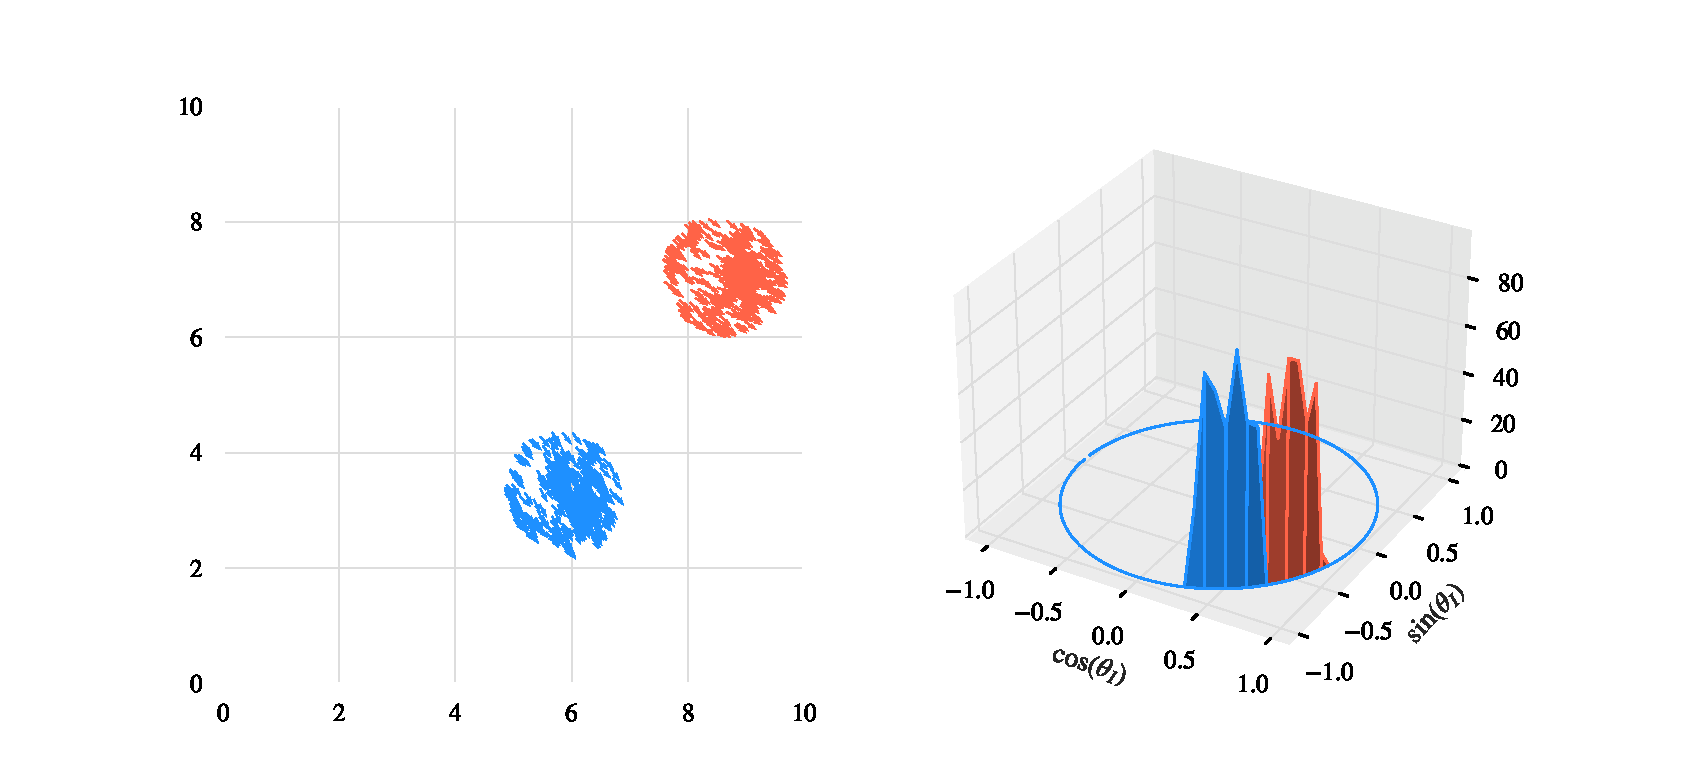
\includegraphics[width=\textwidth]{./figs/CorrectCoupling_uniform_0.010_2.00.eps}
	\vspace{-1cm}
	\caption{集群态 ($\lambda=0.01, d_0=2, random seed=10$)}
	\label{fig:fig231.3}
\end{figure}

\begin{figure}[H]
	\centering
	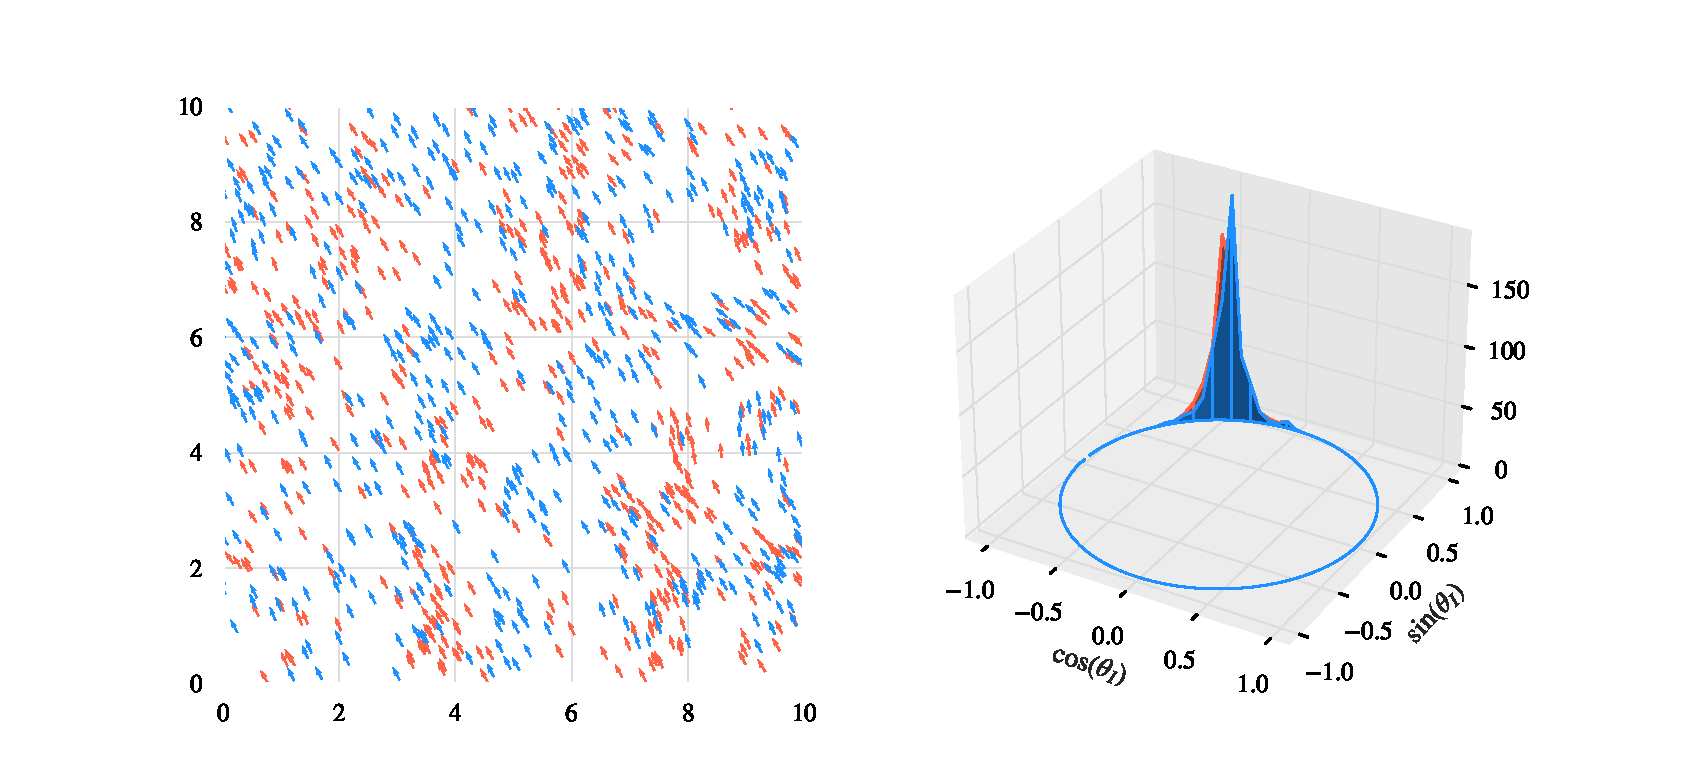
\includegraphics[width=\textwidth]{./figs/CorrectCoupling_uniform_0.600_3.00.eps}
	\vspace{-1cm}
	\caption{快速取向一致 ($\lambda=0.6, d_0=3, random seed=10$)}
	\label{fig:fig231.4}
\end{figure}

当粒子处于集群态或快速取向一致时,相位单位圆的分布如图\ref{fig:fig231.3}和图\ref{fig:fig231.4}所示. 这两种状态的相位同步的程度较高.

\subsubsection{粒子旋转中心的坐标}

\begin{figure}[H]
	\centering
	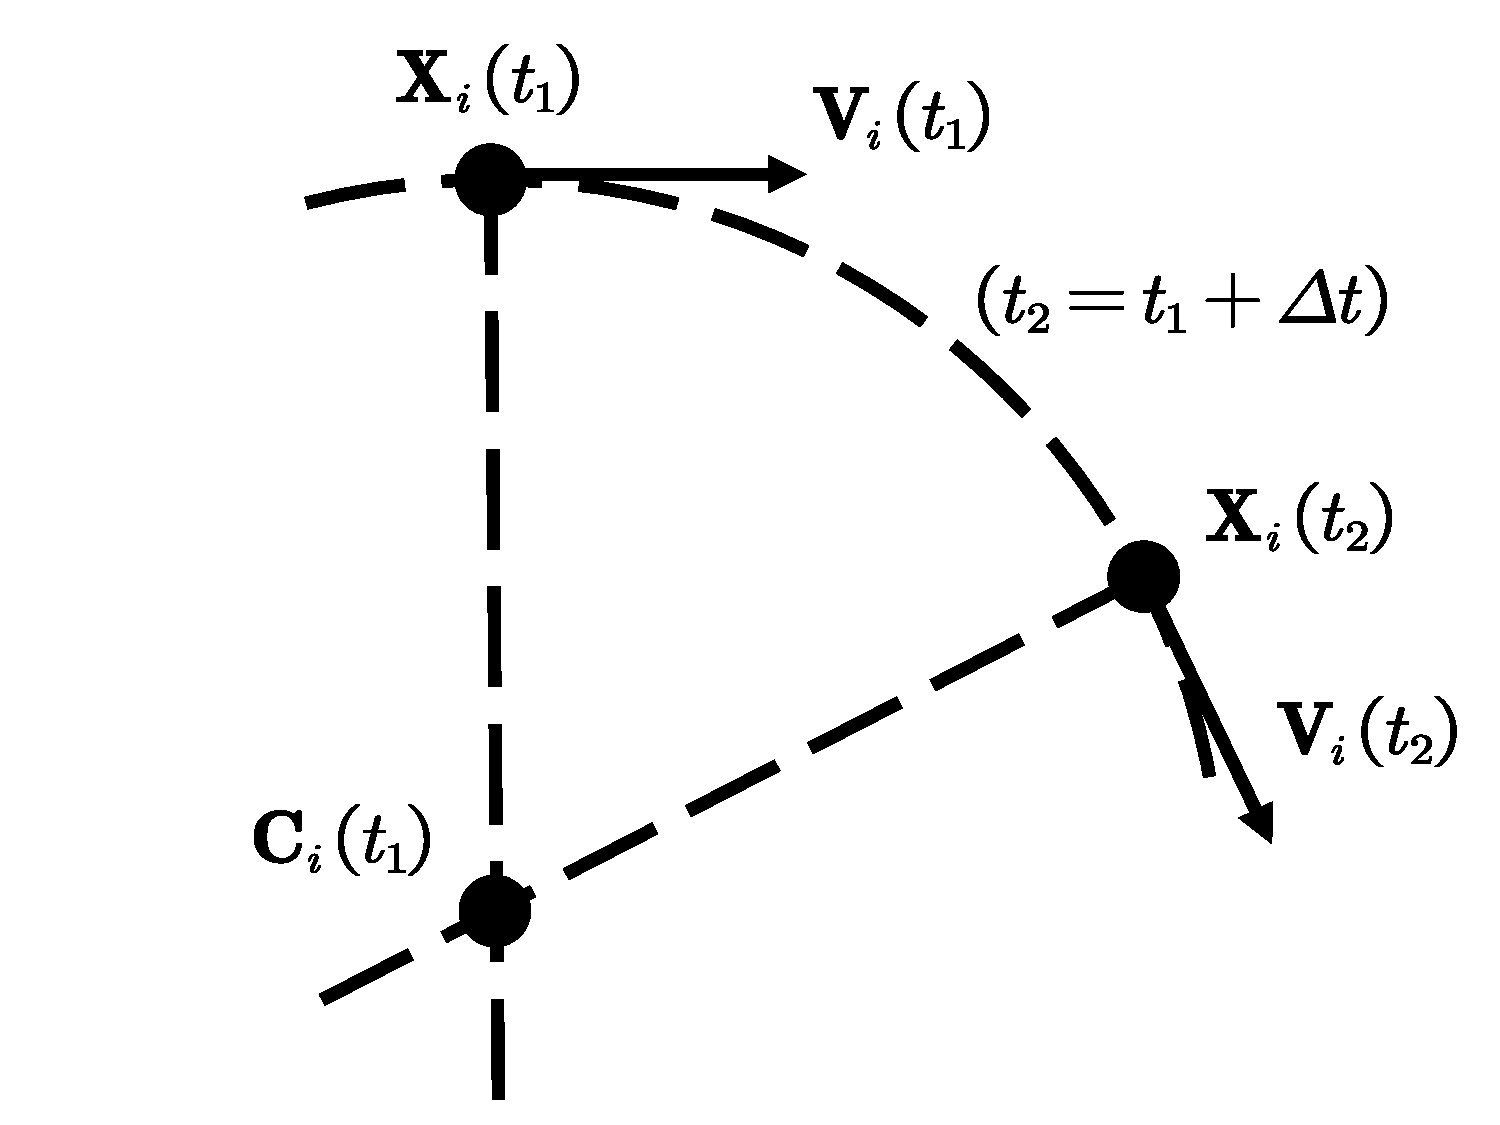
\includegraphics[width=0.3\textwidth]{./figs/旋转圆心示意图.pdf}
	\vspace{-0.2cm}
	\caption{旋转圆心示意图}
	\label{fig:fig232.1}
\end{figure}

如图 \ref{fig:fig232.1} 所示,对于任意粒子$i$, 其当前坐标为$\mathbf{X}_i\left( t_1 \right)$, 速度为$\mathbf{V}_i\left( t_1 \right)$, 下一时刻的坐标为$\mathbf{X}_i\left( t_2 \right)$, 速度为$\mathbf{V}_i\left( t_2 \right)$, 则其旋转中心坐标为两个时刻法向量所在直线的交点, 假设旋转中心坐标为$\mathbf{C}_i\left( t_1 \right)$, 则有

\vspace{-0.5cm}

$$
\begin{cases}
	\mathbf{C}_i\left( t_1 \right) \cdot \mathbf{V}_i\left( t_1 \right) =\mathbf{X}_i\left( t_1 \right) \cdot \mathbf{V}_i\left( t_1 \right) \\
	\mathbf{C}_i\left( t_1 \right) \cdot \mathbf{V}_i\left( t_2 \right) =\mathbf{X}_i\left( t_2 \right) \cdot \mathbf{V}_i\left( t_2 \right) \\
\end{cases}
$$

% 对于任意的粒子$i$,其当前坐标为$\left( x_i,y_i \right)$,相速度为$\dot{\theta}_i$,假设从当前时刻开始,其相速度不变,即$\dot{\theta}_i$为常数,记录该粒子在一个周期($2\pi$)内的运动轨迹,即$2\pi / \dot{\theta}_i$时间内,以当前坐标$\left( x_i,y_i \right)$为起点,以$\left\{ v\cos \theta _i,v\sin \theta _i \right\} $为速度,运动得到的轨迹,以轨迹上点坐标的算数平均作为该粒子的旋转中心坐标,即

% $$
% \begin{cases}
% 	\bar{x}_i=\frac{1}{2\pi / \dot{\theta}_i}\int_{0}^{2\pi / \dot{\theta}_i}{\left[ x_i+v\cos\left( \theta_i + \dot{\theta}_i \cdot t \right)\right] dt}\\
% 	\bar{y}_i=\frac{1}{2\pi / \dot{\theta}_i}\int_{0}^{2\pi / \dot{\theta}_i}{\left[ x_i+v\sin\left( \theta_i + \dot{\theta}_i \cdot t \right)\right] dt}\\
% \end{cases}
% $$

求解上述方程组,可以得到每个粒子的旋转中心坐标,如下图\ref{fig:fig232.2}:% \ref{fig:fig2}.

\begin{figure}[H]
	\centering
	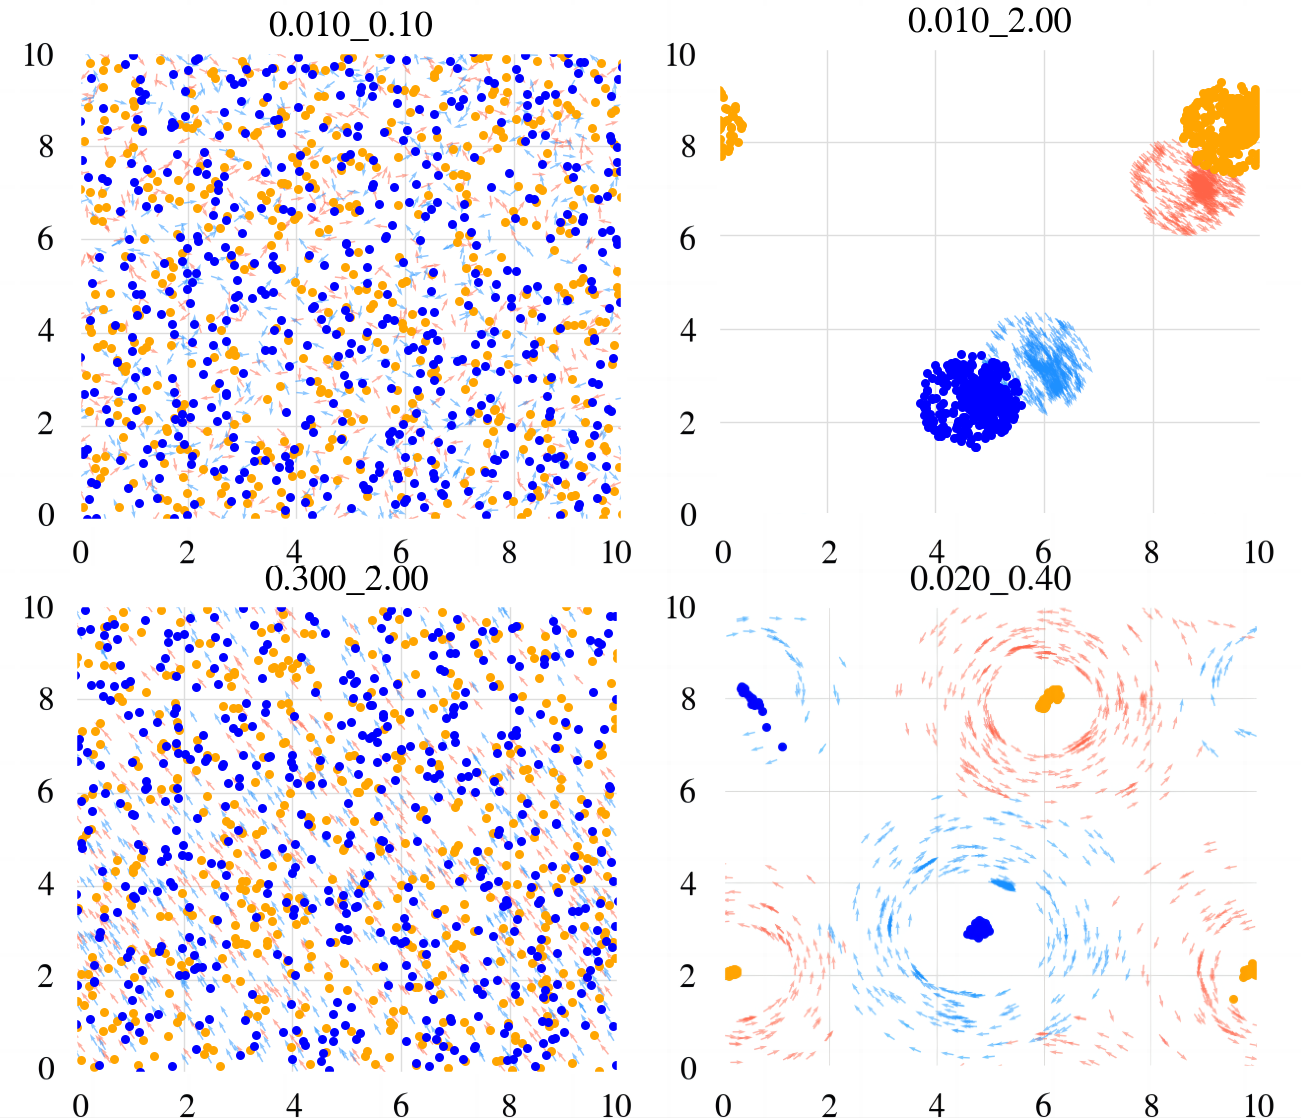
\includegraphics[width=0.7\textwidth]{./figs/centorsBigGraph_sub.png}
	\vspace{-0.2cm}
	\caption{旋转中心求解结果示例}
	\label{fig:fig232.2}
\end{figure}

上图中,带有箭头的半透明色点表示粒子,光滑实心色点表示粒子的旋转中心,其中,橙色点为正手性粒子(半透明红色箭头)的旋转中心,蓝色点为负手性粒子(半透明蓝色箭头)的旋转中心. 从图中可以看出,形成清晰的环态后,环上粒子的旋转中心较为集中,说明同一环上粒子的运动规律较为接近,且近似圆周运动.



\subsubsection{基于调整耦合距离的聚类算法}

考虑到粒子在形成环态或集群态时,会形成多个环或集群,因此可以对粒子进行聚类从而计算各环或群的局部序参量. 由于环在欧氏空间中的分布较为特殊(中空,环与环相邻),因此改为对粒子的旋转中心进行聚类. 此外,周期性边界条件会导致粒子的旋转中心跨边界,这里采样式\ref{eq:eq1}对旋转中心坐标进行调整.

\begin{algorithm}
	\SetKw{in}{in}
	\SetKwData{Left}{left}\SetKwData{This}{this}\SetKwData{Up}{up}
	\SetKwFunction{Union}{Union}\SetKwFunction{FindCompress}{FindCompress}
	\SetKwInOut{Input}{input}\SetKwInOut{Output}{output}

	\BlankLine
	\KwData{A set $S=\left\{(\bar{x}_i, \bar{y}_i)\right\}$ of particles' circular center coordinates}
	\KwIn{cluster distance $d_{th}$}
	\KwResult{A cluster set $C=\left\{
		\left\{ 1 \right\}
	 \right\}$}
	% \BlankLine
	\emph{$C$ $\leftarrow$ $\left\{(\bar{x}_1, \bar{y}_1)\right\}$}\;
	\For{$i\leftarrow 2$ \KwTo $N$}{\label{forins}
		\For{class set $C_k$ \in $C$}{
			\For{$j$ \in $C_k$}{
				\If(\tcp*[f]{belong to $C_k$}){$\bar{d}_{ij} < d_{th}$}{
					$C_j \leftarrow C_j \cup \left\{i\right\}$\;
					go to line \ref{forins}\;
				}
			}
		}
		$C \leftarrow C \cup \left\{\left\{i\right\}\right\}$; \tcp*[f]{create new class}
	}
	\caption{Clustering algorithm based on adjusted distance}\label{algo_disjdecomp}
\end{algorithm}\DecMargin{1em}

执行该算法后,可以得到如下图\ref{fig:fig233.1}所示的聚类结果. 对比左侧子图与右侧子图,可以发现,算法可以较好地将多个环分开.

\begin{figure}[H]
	\centering
	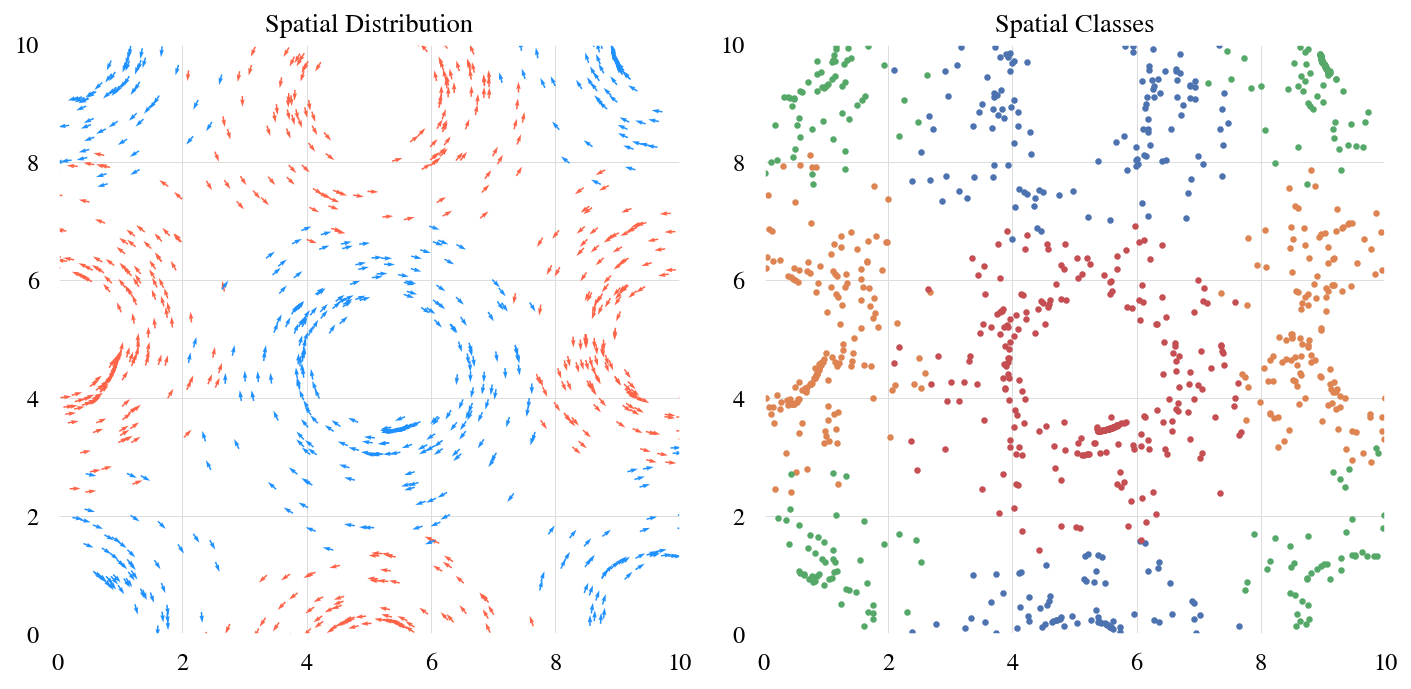
\includegraphics[width=0.9\textwidth]{./figs/ClusteringResult.png}
	\vspace{-0.4cm}
	\caption{聚类结果 ($d_{th}=1, \lambda=0.02, d_0=0.4, random seed=80$)}
	\label{fig:fig233.1}
\end{figure}

\subsubsection{序参量的定义与计算}

% \textbf{旋转中心距离原点的距离标准差(截面序参量)}

% $$
% \sigma _d=\sqrt{\frac{1}{N}\sum_{i=1}^{N}{\left( d_i-\bar{d} \right) ^2}}
% $$

% \begin{figure}[H]
% 	\centering
% 	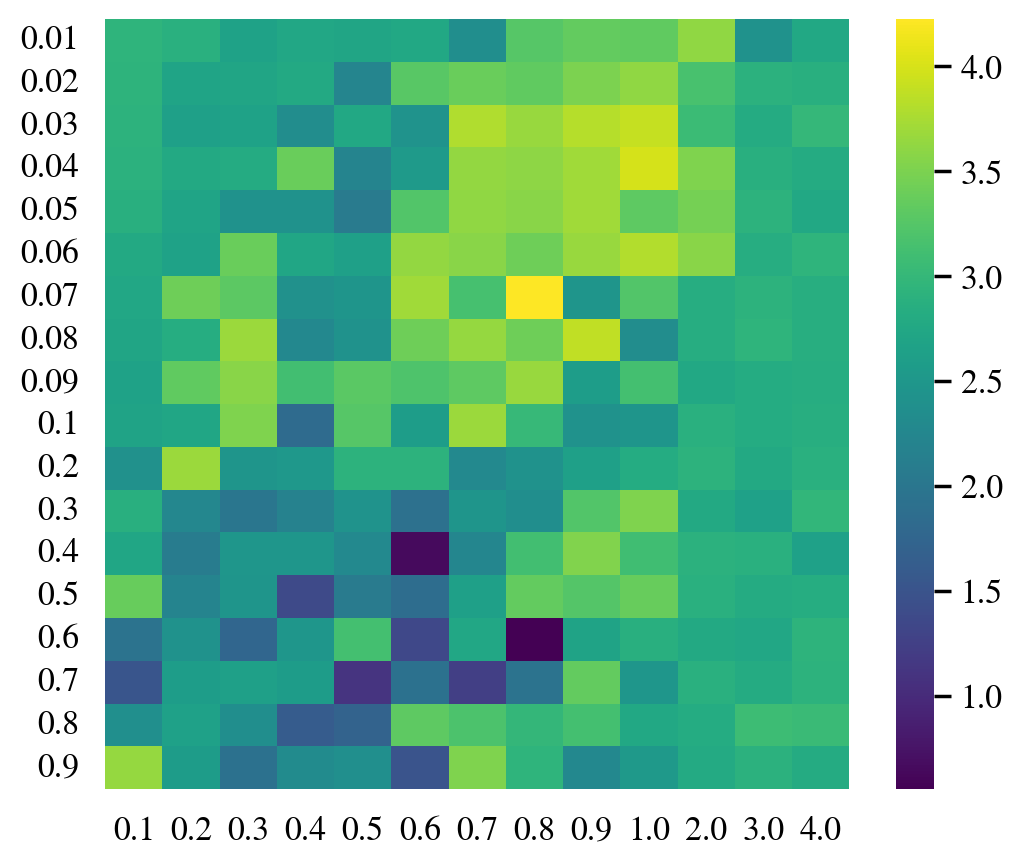
\includegraphics[width=0.7\textwidth]{./figs/stdd.jpg}
% 	\caption{旋转中心原点距离标准差}
% 	\label{fig:fig12}
% \end{figure}

\textbf{旋转中心邻域内的其余中心数(截面序参量)}

$$
N_{nearby}=\frac{1}{N}\sum_{i=1}^N{\left( \sum_{j=1}^N{\left[ \bar{d}_{ij}<\bar{d}_{ij}^{th} \right]} \right)}, 
$$

其中,$\bar{d}_{ij}^{th}$为阈值,取$\bar{d}_{ij}^{th}=1$.

\begin{figure}[H]
	\centering
	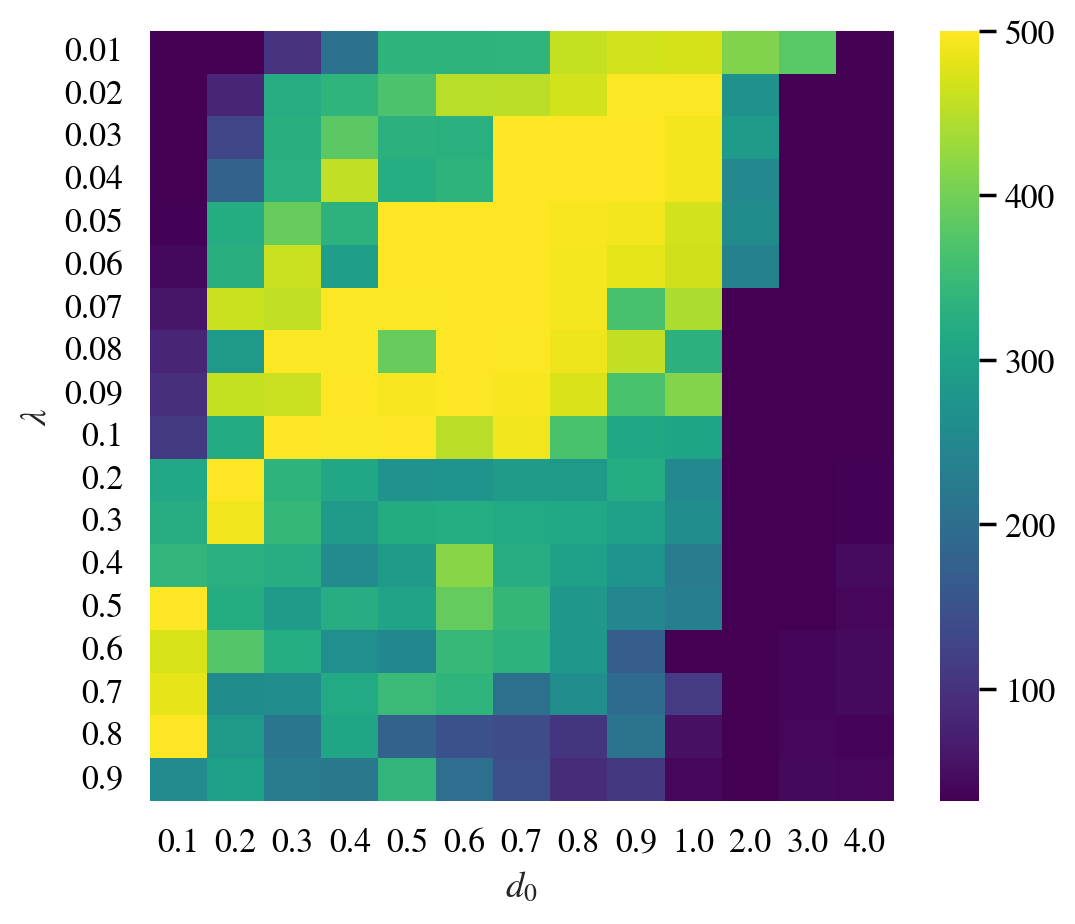
\includegraphics[width=0.7\textwidth]{./figs/nearbyNums.png}
	\caption{旋转中心邻域内的其余中心数}
	\label{fig:fig234.1}
\end{figure}

观察图\ref{fig:fig234.1},可以发现,该序参量可以较好地将空间当中的聚集情况反映出来.左上角与右下角深色区域的粒子在空间上没有形成聚集,而中间部分的粒子在空间上形成了聚集.此外,集群态的序参量取值比环态的序参量取值小,这是因为集群态的旋转中心集中度较低,导致与原点距离的标准差更小.

\newpage
\noindent\textbf{粒子旋转中心坐标(时序序参量)}

考虑到粒子在二维平面上运动,因此该序参量分为$x$坐标和$y$坐标两个分量,将各粒子旋转中心坐标以散点图形式分别绘制得到图下图像:

\begin{figure}[H]
	\centering
	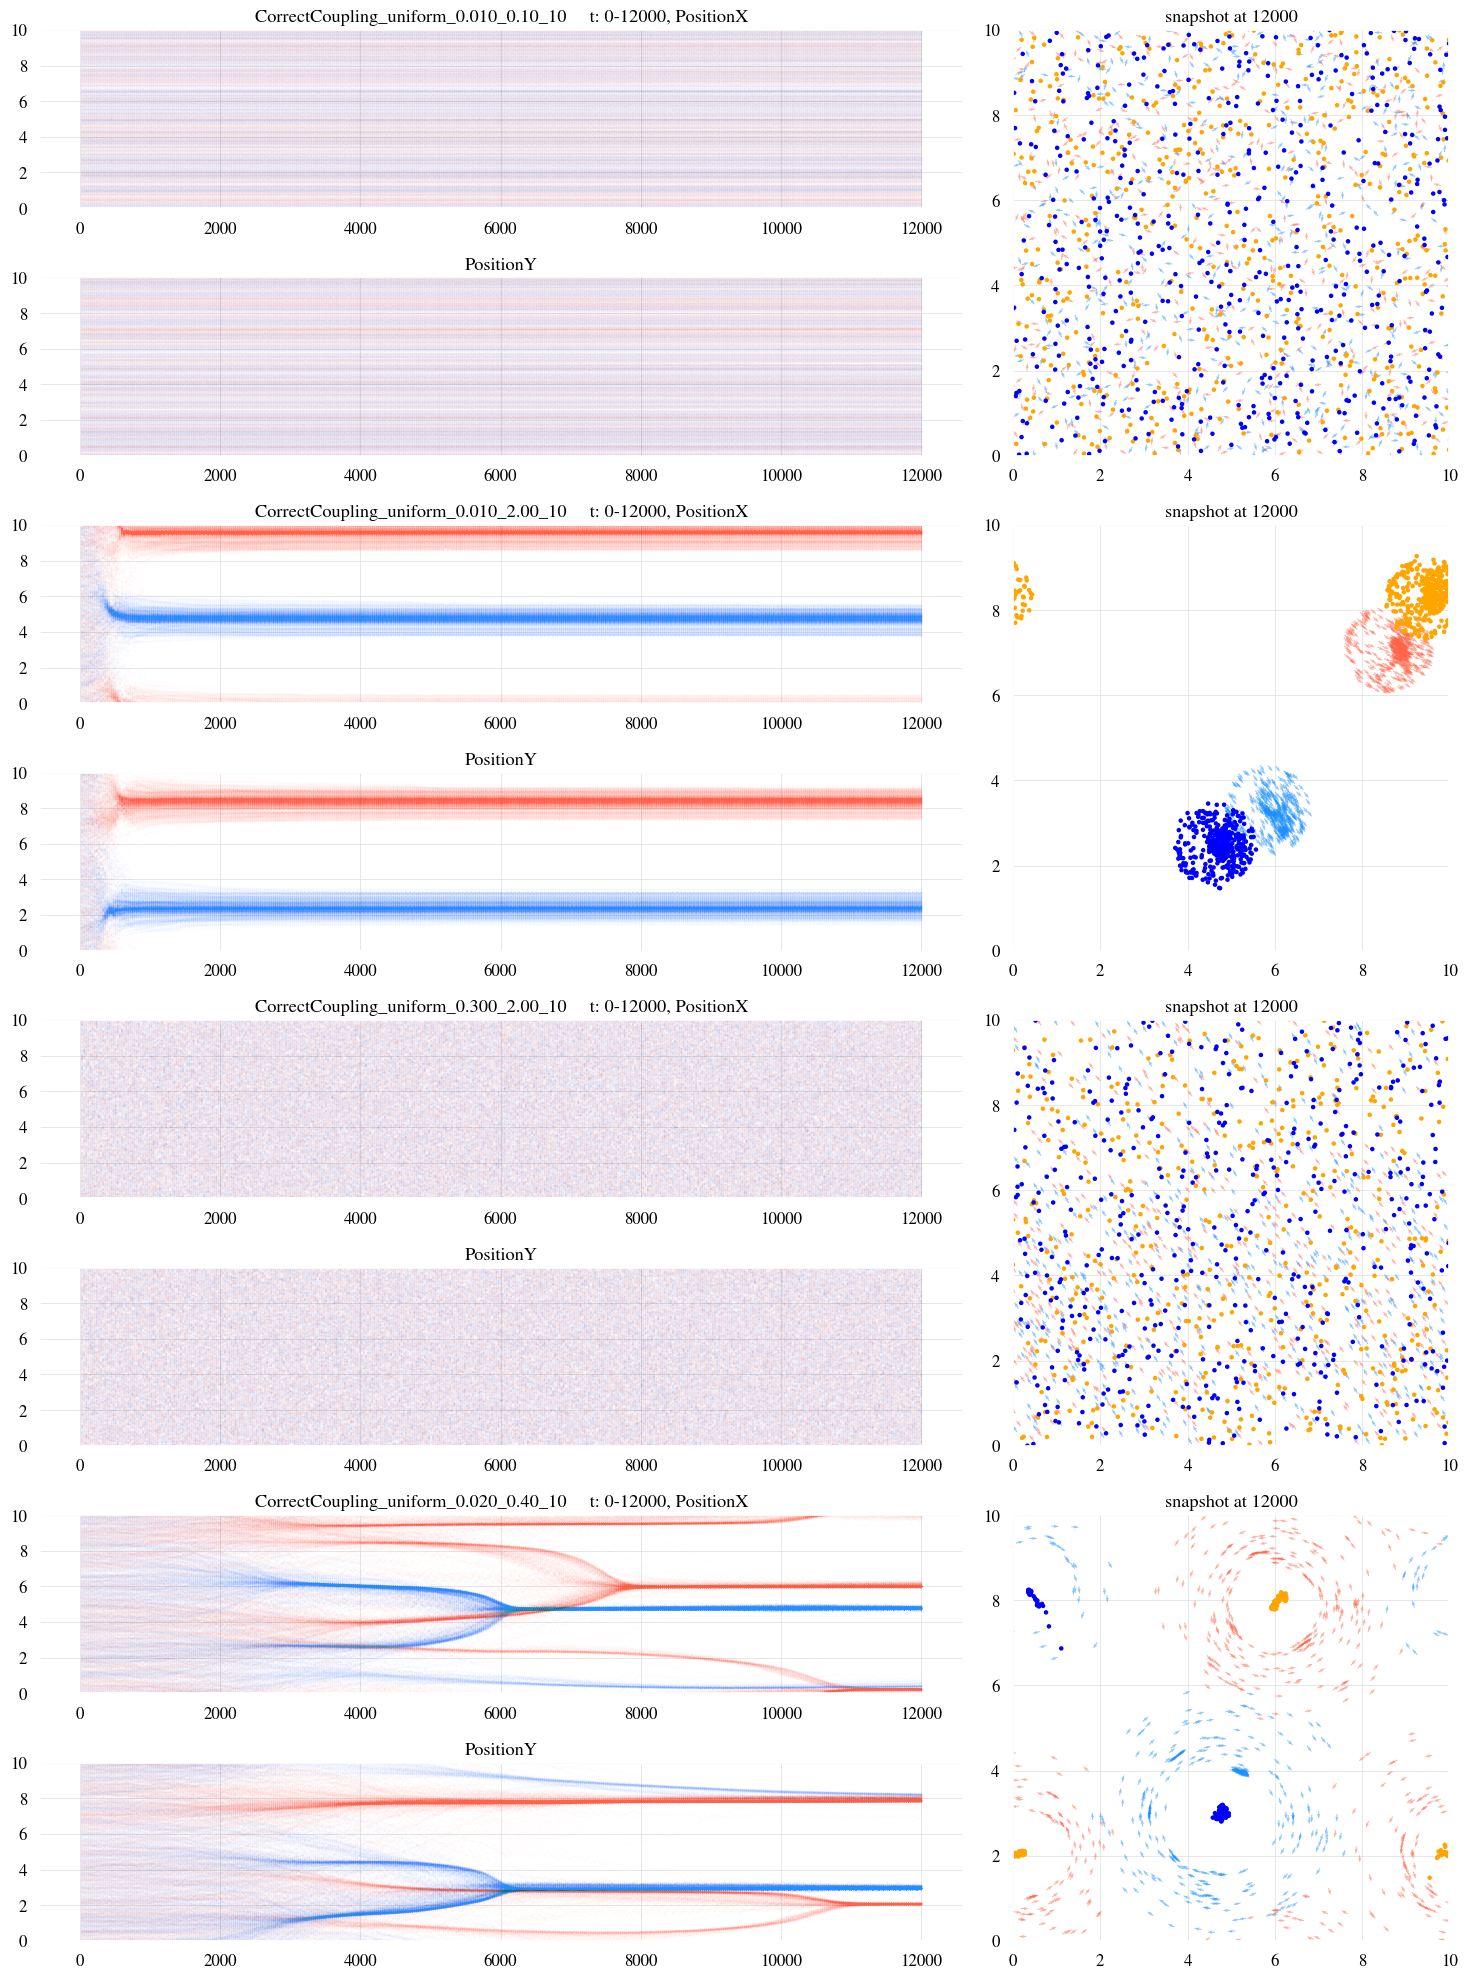
\includegraphics[width=0.9\textwidth]{./figs/totalXY.png}
	\caption{旋转中心坐标}
	\label{fig:fig234.2}
\end{figure}


\newpage
\noindent\textbf{粒子旋转半径(时序序参量)}

% \begin{figure}[H]
% 	\centering
% 	\includegraphics[width=0.8\textwidth]{./figs/globalR.png}
% 	\caption{旋转中心邻域内的其余中心数}
% 	\label{fig:fig234.2}
% \end{figure}

\newpage
\noindent\textbf{聚类旋转半径(时序序参量)}

根据欧式聚类的结果,将所有粒子分为若干类,每一类的旋转半径为该类所有粒子的旋转半径的算数平均,即

$$
\bar{R}_c=\frac{1}{N_c}\sum_{i=1}^{N_c}{\bar{r}_i},\ (N_c\ge N_{th})
$$

其中,$N_c$为第$c$类的粒子数. 此外,为防止空间当中出现孤立的粒子,将粒子数小于某一阈值的类剔除,这里,$N_{th}$为阈值,取$N_{th}=5$.

% \begin{figure}[H]
% 	\centering
% 	\includegraphics[width=0.8\textwidth]{./figs/clusterR.png}
% 	\caption{旋转中心邻域内的其余中心数}
% 	\label{fig:fig234.3}
% \end{figure}

\newpage
\noindent\textbf{聚类中心坐标(时序序参量)}

考虑到粒子在二维平面上运动,因此该序参量分为$x$坐标和$y$坐标两个分量,即

$$
\bar{x}_c=\frac{1}{N_c}\sum_{i=1}^{N_c}{\bar{x}_i},\quad \bar{y}_c=\frac{1}{N_c}\sum_{i=1}^{N_c}{\bar{y}_i},\ (N_c\ge N_{th})
$$

% \begin{figure}[H]
% 	\centering
% 	\includegraphics[width=0.8\textwidth]{./figs/clusterXY.png}
% 	\caption{旋转中心邻域内的其余中心数}
% 	\label{fig:fig234.4}
% \end{figure}


% \newpage

% \section{附录}\label{sec:appendix}

% \begin{figure}[H]
% 	\centering
% 	\includegraphics[width=\textwidth]{./figs/centorsBigGraph.png}
% 	\caption{旋转中心}
% 	\label{fig:fig2}
% \end{figure}

% \title{Swarm dynamics for oscillators with Phase Orientation Correlation}
% \maketitle

% \section{Introduction}

% \section{Results}
% \subsection{The Model}
% \subsection{Numerics}
% \subsection{Theoretical Analysis}


\end{document}